\documentclass[13pt,a4paper]{report}
\usepackage[margin=0.6in]{geometry}
\usepackage{fancybox}
\usepackage[utf8]{inputenc}
\usepackage[vietnamese,main=english]{babel}
\usepackage{multicol}
\usepackage{tabularx}
\usepackage{lmodern}
\usepackage{minted}
\usepackage{indentfirst}
\usepackage{float}
\usepackage{enumitem}
\usepackage{afterpage}
\usepackage[super]{nth}
\usepackage{titlesec}
\usepackage{bigdelim}
\usepackage[titles]{tocloft}
\usepackage{makecell}
\usepackage{arydshln}
\usepackage{perpage} %the perpage package
\usepackage{graphicx}
\usepackage{caption}
\usepackage{gensymb}
\usepackage{tikz}
\usepackage{circuitikz}
\usepackage{pgfplots}
\usepackage{cancel}
\usepackage{xurl}
\usepackage[bottom]{footmisc}
\usepackage[font=footnotesize,labelfont={scriptsize}]{subfig}
\usepackage{wrapfig}
\usepackage{latexsym,amssymb,amsmath}
%\usepackage{algpseudocode}
\usepackage{tocvsec2}
\usepackage{fancyref}
\usepackage{bookmark}
\usepackage{hyperref}
\usepackage[nameinlink,noabbrev]{cleveref}

\newcolumntype{Y}{>{\centering\arraybackslash}X}

\PassOptionsToPackage{hyphens}{url}

\makeatletter
\pgfcircdeclarebipole{}{\ctikzvalof{bipoles/vsourceam/height}}{vsourceAM}{\ctikzvalof{bipoles/vsourceam/height}}{\ctikzvalof{bipoles/vsourceam/width}}{%
  \pgfsetlinewidth{\pgfkeysvalueof{/tikz/circuitikz/bipoles/thickness}\pgfstartlinewidth}
   \pgfpathellipse{\pgfpointorigin}{\pgfpoint{0}{\pgf@circ@res@up}}{\pgfpoint{\pgf@circ@res@left}{0}}
   \pgfusepath{draw}
   \pgfscope
       \pgftransformxshift{0.6*\ctikzvalof{bipoles/vsourceam/margin}\pgf@circ@res@left}
       \pgftext[rotate=-\pgf@circ@direction]{$+$}
       \pgfusepath{draw}
   \endpgfscope
   \pgfscope
       \pgftransformxshift{0.6*\ctikzvalof{bipoles/vsourceam/margin}\pgf@circ@res@right}
       \pgftext[rotate=-\pgf@circ@direction]{$-$}
       \pgfusepath{draw}
   \endpgfscope
}
\makeatother

\MakePerPage{footnote} %the perpage package command
\usetikzlibrary{shapes,positioning,arrows,calc}

\newcommand*\justify{%
  \fontdimen2\font=0.4em% interword space
  \fontdimen3\font=0.2em% interword stretch
  \fontdimen4\font=0.1em% interword shrink
  \fontdimen7\font=0.1em% extra space
  \hyphenchar\font=`\-% allowing hyphenation
}
\renewcommand\cftchapafterpnum{\vskip-2pt}
\renewcommand\cftsecafterpnum{\vskip-2pt}

\renewcommand{\theequation}{\arabic{equation}}

% FLOW CHART
\tikzstyle{startstop} = [rectangle, rounded corners, minimum width=3cm, minimum height=1cm,text centered, draw=black, fill=red!30]
\tikzstyle{io} = [trapezium, trapezium left angle=70, trapezium right angle=110, minimum width=3cm, minimum height=1cm, text centered, draw=black, fill=blue!30]
\tikzstyle{process} = [rectangle, minimum width=3cm, minimum height=1cm, text centered, draw=black, fill=orange!30, text width=4cm]
\tikzstyle{decision} = [diamond, aspect=2.5, minimum width=3cm, minimum height=1cm, text centered, draw=black, fill=green!30]
\tikzstyle{arrow} = [thick,->,>=stealth]

% CHAPTER FORMAT
\titleformat{\chapter}%[display]
{\bfseries\fontsize{25}{30}\selectfont\raggedright}% Format and size of title text
{\llap{%
    \rule[-6pt]{6cm}{1.18cm}\rule{6pt}{0pt}}% Black box to the left, lowered 6pt. The end rule is a horisontal space.
  \llap{% Number also to the left, on top of the black box.
    \fontsize{30}{44}\selectfont\color{white}\thechapter\rule{10pt}{0pt}}}{0pt}{}{}

\counterwithin{figure}{section}
\renewcommand{\thefigure}{\arabic{chapter}.\arabic{section}.\alph{figure}}

\renewcommand{\thetable}{\arabic{table}}

\renewcommand\labelitemi{$-$}
  
\titleformat{\section}
  {\LARGE\bfseries}{}{}{}
\renewcommand\thesection{\arabic{section}.}
\renewcommand\thesubsection{\arabic{subsection}}
\makeatletter
\renewcommand*\l@section{\@dottedtocline{1}{1.5cm}{2em}}
\renewcommand\section{\@startsection {section}{1}{-1em}%
  {-3.5ex \@plus -1ex \@minus -.2ex}%
  {2.3ex \@plus.2ex}%
  {\normalfont\Large\bfseries}}
\def\sectionmark#1{%
      \markright {\MakeUppercase{#1}}}
\makeatother

\titleformat{\subsection}
  {\normalfont\bfseries}{\thesubsection.}{0.5em}{}
\renewcommand\cftsubsecaftersnum{.} 
\renewcommand\thesubsection{\alph{subsection}}

\addto{\captionsenglish}{%
  \renewcommand{\bibname}{References}
}

%\addtocontents{toc}{\setcounter{tocdepth}{2}}
%\addtocontents{lof}{\vskip -1.6cm}
%\addtocontents{lot}{\vskip -1.6cm}
    
% TOC settings
\renewcommand\cftchapnumwidth{2.8em}
\renewcommand\cftsecnumwidth{3em}
\renewcommand\cftsecindent{3em}
\renewcommand\cftsubsecindent{5em}
\renewcommand\thechapter{\Roman{chapter}}
    
%\titleformat{\chapter}[display]{\normalfont\huge\bfseries}{}{0pt}{\Huge}
\newcommand{\hsp}{\hspace{20pt}}
%\titleformat{\chapter}[hang]{\Huge\bfseries}{\thechapter\hsp\textcolor{gray75}{|}\hsp}{0pt}{\Huge\bfseries}
\titleformat*{\subsubsection}{\large\bfseries}
%\titlespacing*{\chapter}{0pt}{0pt}{0pt}
    
\newcolumntype{P}[1]{>{\centering\arraybackslash}p{#1}}
\newcolumntype{C}{>{\centering\arraybackslash}p{4em}}
    
\setlist[itemize]{noitemsep, topsep=0pt}
%\AtBeginEnvironment{multicols}{\RaggedRight}

\titlespacing*{\chapter}{0pt}{0pt}{20pt}

\newcommand\Chapter[2]{\chapter
  [#1\text{: }\hfil\hbox{}\protect\linebreak{\itshape#2}]%
  {#1\\[-0.75ex]\Large#2}%
  \markboth{\MakeUppercase{\chaptername\ \thechapter.\ #1}}{}%
}


\def\doubleoverline#1{\overline{\overline{#1}}}

\begin{document}
%Trang bìa 1
\fontsize{13pt}{18pt}\selectfont
\begin{titlepage}
\thispagestyle{empty}
\thisfancypage{%đóng khung trang này
\setlength{\fboxsep}{0pt}% 8pt là độ dày của đường viền
\fbox}{} % phần nội dung sau là tương tự như đã làm
\

\begin{center}
\begin{large}
HO CHI MINH CITY UNIVERSITY OF TECHNOLOGY $-$ VNU HCMC
\end{large} \\
\begin{large}
OFFICE FOR INTERNATIONAL STUDY PROGRAM
\end{large} \\
\begin{large}
FACULTY OF ELECTRICAL AND ELECTRONIC ENGINEERING
\end{large} \\
\textbf{--------------------  *  --------------------}\\[4cm]
\includegraphics[scale=0.1]{logobk.png}\\[1cm]
{\fontsize{20pt}{1}\selectfont DIGITAL SYSTEMS (LAB)}\\
{\fontsize{20pt}{1}\selectfont EXPERIMENTAL REPORT (Prelab 1)}\\[2.5cm]
\end{center}

\begin{otherlanguage}{vietnamese}
\begin{tabbing}
	\hspace{3.5cm}Lecturer  \ \ \ \ \=: \textbf{\parbox[t]{9cm}{Mr. Nguyễn Tuấn Hùng}}\\
	\hspace{3.5cm}Subject \>: \textbf{\parbox[t]{12cm}{Digital Systems}}\\
	\hspace{3.5cm}Class \>: \textbf{\parbox[t]{9cm}{TT06}}\\
	\hspace{3.5cm}Name \>: \textbf{\parbox[t]{9cm}{
		Lương Triển Thắng}}\\
	\hspace{3.5cm}Student ID \>: \textbf{\parbox[t]{9cm}{
		2051194}}\\[40pt]
\end{tabbing}
\end{otherlanguage}

\vspace{2.25cm}
\begin{center}
{\fontsize{13pt}{1}\selectfont Ho Chi Minh City, \nth{31} May, 2022}
\end{center}
\end{titlepage}

\tableofcontents

\setminted{fontsize=\normalsize}

\setcounter{chapter}{0}

\Chapter{Laboratory 1}{Get started with FPGA}
\section{Get started with FPGA}
\ctikzset{logic ports=ieee}
\begin{center}
LEDR(9) $<$= SW(9);\\
LEDR(8) $<$= SW(8);\\
...\\
LEDR(0) $<$= SW(0);
\end{center}

\subsection*{Code}
\begin{minted}{vhdl}
LIBRARY IEEE;
USE IEEE.STD_LOGIC_1164.ALL;

ENTITY Exc1 IS
	PORT (
		SW : IN STD_LOGIC_VECTOR(9 DOWNTO 0);
		LEDR : OUT STD_LOGIC_VECTOR(9 DOWNTO 0)
	);
END ENTITY;

ARCHITECTURE behavior OF Exc1 IS
BEGIN
	LEDR <= SW;
END ARCHITECTURE;
END Logic;
\end{minted}

\section{Know how to program one-bit wide 2-to-1 multiplexer}

\begin{center}
m $<$= (NOT (s) AND x) OR (s AND y)
\end{center}

\ctikzset{logic ports=ieee}
\begin{figure}[H]
\centering
\begin{circuitikz}
\draw
  (2,0) node[and port] (and1) {}
  (2,-3) node[and port] (and2) {}
  (5,-1.5) node[or port] (or) {}
  
  (-0.1, -1.5) node[scale=0.5, not port, rotate=90](not) {}
  ;
  
\draw 
  (and1.out) |- (or.in 1)
  (and2.out) |- (or.in 2)
  
  (and1.in 1) -- ++(-2,0) node[anchor=east] {$x$}
  (and2.in 1) -- ++(-2,0) node[anchor=east] {$s$}
  (and2.in 2) -- ++(-2,0) node[anchor=east] {$y$}
  
  (and2.in 1) to [open, -*] ++(-1,0) -- (not.in)
  (not.out) |- (and1.in 2)
  
  (or.out) -- ++(1,0) node[anchor=west] {$m$}
    ;
\end{circuitikz}
\caption{Circuit diagram}
\end{figure}

\begin{figure}[H]
\centering
\begin{circuitikz}
\tikzset{mux21/.style={muxdemux, muxdemux def={NL=2, NB=0, NT=1, NR=1, Lh=6, Rh=3, w=1.5}}}

\draw
  (0,0) node[mux21] (mux21) {}
  
  (mux21.lpin 1) -- ++(-1,0) node[anchor=east] {$x$}
  (mux21.lpin 2) -- ++(-1,0) node[anchor=east] {$y$}
  (mux21.rpin 1) -- ++(1,0) node[anchor=west] {$m$}
  (mux21.tpin 1) -- ++(0,1) node[anchor=south] {$s$}
  ;
  
\draw 
  
    ;
\end{circuitikz}
\caption{Circuit diagram}
\end{figure}


\subsection{Code}
\begin{minted}{vhdl}
LIBRARY ieee;
USE ieee.std_logic_1164.ALL;
ENTITY Exc2 IS
	PORT (
		x : IN std_logic;
		s : IN std_logic;
		y : IN std_logic;
		m : OUT std_logic
	);
END ENTITY;

ARCHITECTURE arch OF Exc2 IS
BEGIN
	m <= (NOT(s) AND x) OR (s AND y);
END arch;
\end{minted}

\subsection{Waveform}
\begin{figure}[H]
\centering
\includegraphics[scale=0.8]{images/Exc2_waveform.png}
\end{figure}

\subsection{Result of RTL viewer}
\begin{figure}[H]
\centering
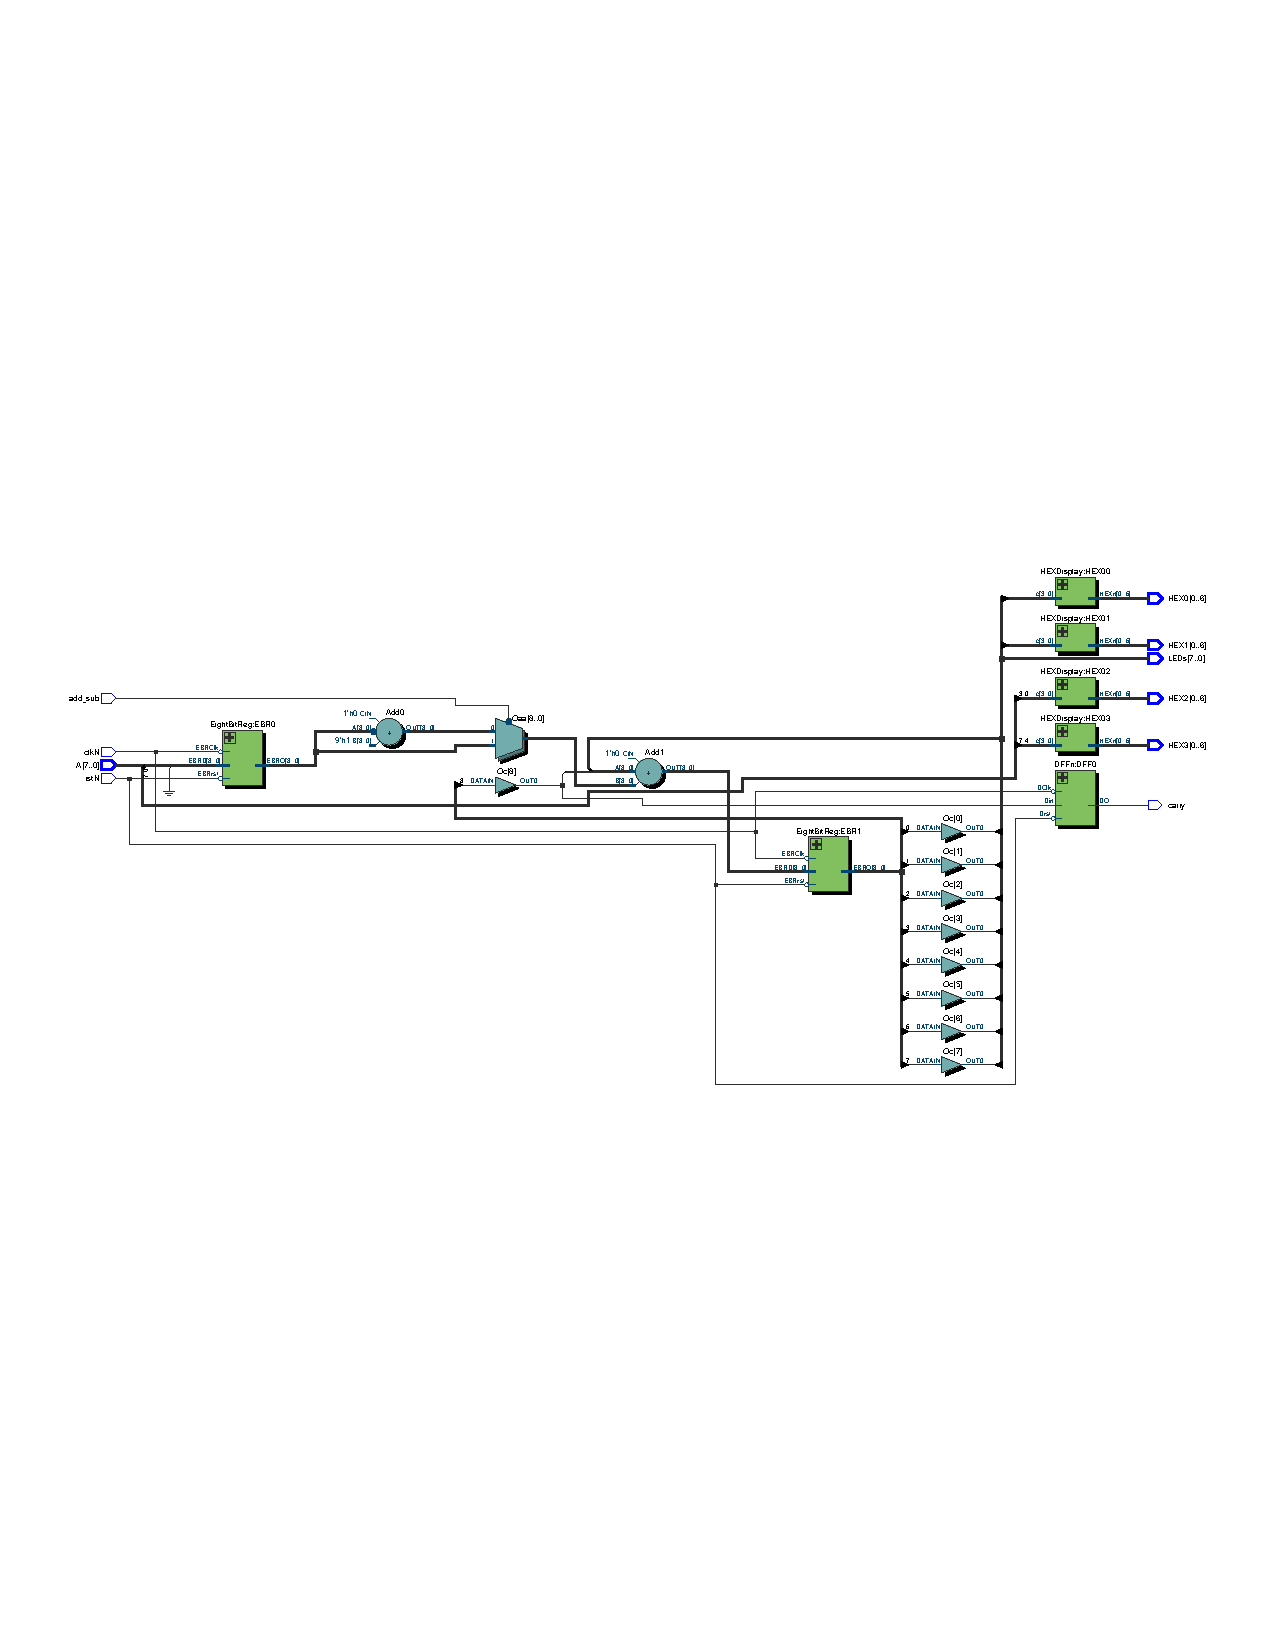
\includegraphics[scale=0.5, clip, trim={2cm 4cm 2cm 6cm}]{images/Exc2_RTL.pdf}
\end{figure}

\section{Know how to interface with 7-segment LED}

\begin{table}[H]
\centering
\begin{tabular}{cc|c|c}
$c_1$ & $c_0$ & HEX0 & LED                                                                                                                                                                                                                         \\ \hline
0     & 0     &  0 1 1 1 1 0 1    & \begin{circuitikz}\ctikzset{seven seg/width=0.25, seven seg/thickness=3pt}\draw (0,0) node[seven segment val=d dot none box off]{};\end{circuitikz} \\
0     & 1     &  1 0 0 1 1 1 1    & \begin{circuitikz}\ctikzset{seven seg/width=0.25, seven seg/thickness=3pt}\draw (0,0) node[seven segment val=E dot none box off]{};\end{circuitikz} \\
1     & 0     &  0 1 1 0 0 0 0    & \begin{circuitikz}\ctikzset{seven seg/width=0.25, seven seg/thickness=3pt}\draw (0,0) node[seven segment val=1 dot none box off]{};\end{circuitikz} \\
1     & 1     &  1 1 1 1 1 1 0    & \begin{circuitikz}\ctikzset{seven seg/width=0.25, seven seg/thickness=3pt}\draw (0,0) node[seven segment val=0 dot none box off]{};\end{circuitikz} \\
\end{tabular}
\end{table}

\subsection{Code}
\begin{minted}{vhdl}
LIBRARY ieee;
USE ieee.std_logic_1164.ALL;

ENTITY Exc3 IS
	PORT (
		c : IN std_logic_vector(1 DOWNTO 0);
		HEX0 : OUT std_logic_vector(0 TO 6)
	);
END Exc3;

ARCHITECTURE behavior OF Exc3 IS
	SIGNAL HEX : std_logic_vector(0 TO 6);
BEGIN
	HEX0 <= NOT(HEX); -- 7SEGLED is active low.
	WITH c SELECT
	HEX <= "0111101" WHEN "00", 
	       "1001111" WHEN "01", 
	       "0110000" WHEN "10", 
	       "1111110" WHEN "11", 
	       "0000000" WHEN OTHERS;
END behavior;
\end{minted}

\subsection{Waveform}
\begin{figure}[H]
\centering
\includegraphics[scale=0.8]{images/Exc3_waveform.png}
\end{figure}

\subsection{Result of RTL viewer}
\begin{figure}[H]
\centering
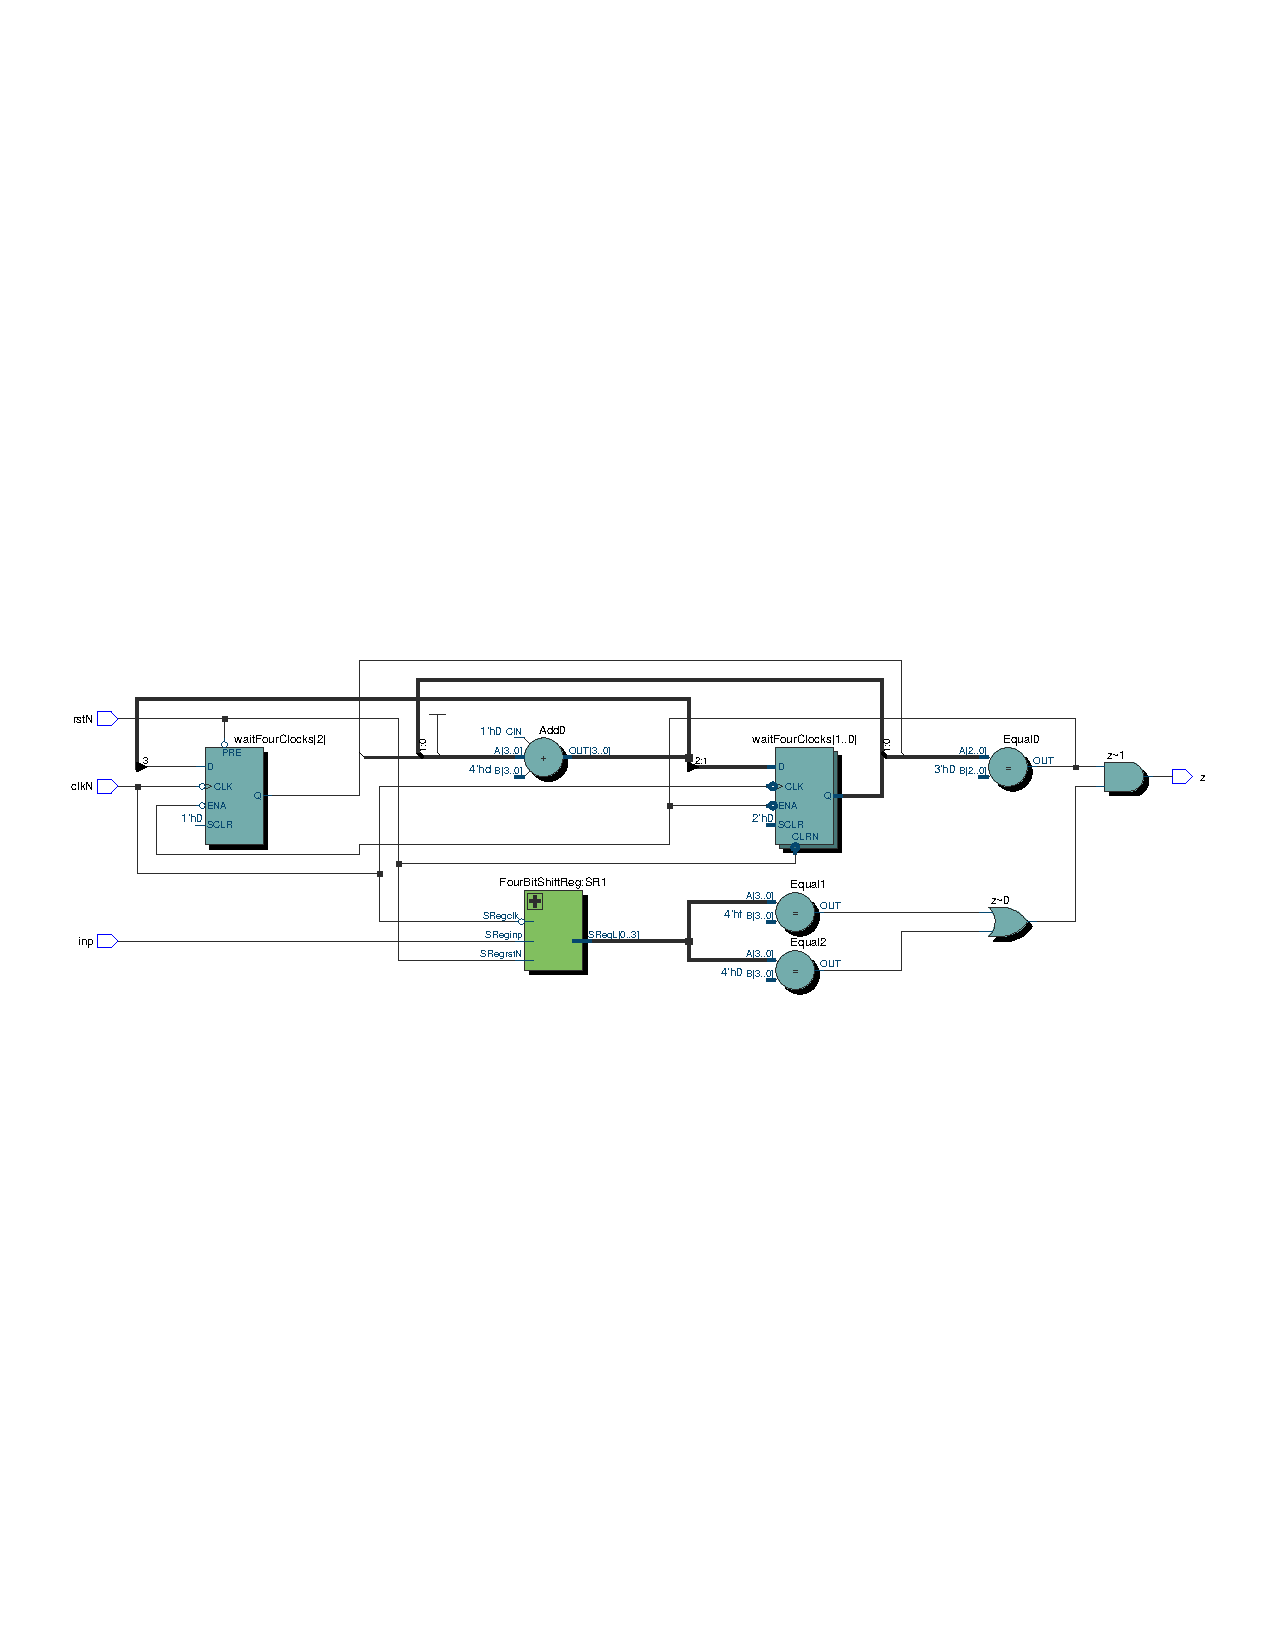
\includegraphics[scale=0.7, clip, trim={2cm 4cm 2cm 3cm}]{images/Exc3_RTL.pdf}
\end{figure}

\end{document}